\documentclass[10pt,pdf,hyperref={unicode}]{beamer}

\mode<presentation>
{
\usetheme{boxes}
\beamertemplatenavigationsymbolsempty

\setbeamertemplate{footline}[page number]
\setbeamersize{text margin left=0.5em, text margin right=0.5em}
}

\usepackage[utf8]{inputenc}
\usepackage[english, russian]{babel}
\usepackage{bm}
\usepackage{multirow}
\usepackage{ragged2e}
\usepackage{indentfirst}
\usepackage{multicol}
\usepackage{subfig}
\usepackage{amsmath,amssymb}
\usepackage{enumerate}
\usepackage{mathtools}
\usepackage{comment}
\usepackage{multicol}

\usepackage[all]{xy}

\usepackage{tikz}
\usetikzlibrary{positioning,arrows}

\tikzstyle{name} = [parameters]
\definecolor{name}{rgb}{0.5,0.5,0.5}

\usepackage{caption}
\captionsetup{skip=0pt,belowskip=0pt}

\newtheorem{rustheorem}{Теорема}
\newtheorem{russtatement}{Утверждение}
\newtheorem{rusdefinition}{Определение}

% colors
\definecolor{darkgreen}{rgb}{0.0, 0.2, 0.13}
\definecolor{darkcyan}{rgb}{0.0, 0.55, 0.55}

\AtBeginEnvironment{figure}{\setcounter{subfigure}{0}}

\captionsetup[subfloat]{labelformat=empty}

%----------------------------------------------------------------------------------------------------------

\title[Пример слайдов по работе]{Пример слайдов по работе \\ курса}
\author{И.\,О.\,Фамилия}

\institute[]{Московский физико-технический институт}
\date[2022]{\small 10\;февраля\;2022\,г.}

%---------------------------------------------------------------------------------------------------------
\begin{document}

%\begin{frame}
%\titlepage
%\end{frame}

%----------------------------------------------------------------------------------------------------------
%\section{Слайд об исследованиях}
%\begin{frame}{Слайд об исследованиях}
%\bigskip
%Исследуется проблема \ldots.
%\begin{block}{Цель исследования~---}
%предложить метод \ldots.
%\end{block}
%\begin{block}{Требуется предложить}
%\justifying
%\begin{enumerate}[1)]
%\item метод \ldots,
%\item метод \ldots,
%\item метод \ldots.
%\end{enumerate}
%\end{block}
%\begin{block}{Решение}
%Для \ldots.
%end{block}
%\end{frame}

%---------------------------------------------------------------------------------------------------------
\section{One-slide talk }
\begin{frame}{One-slide talk }
GNN + LSTM/GRU

\begin{figure}[h]
\begin{minipage}[h]{0.49\linewidth}
\center{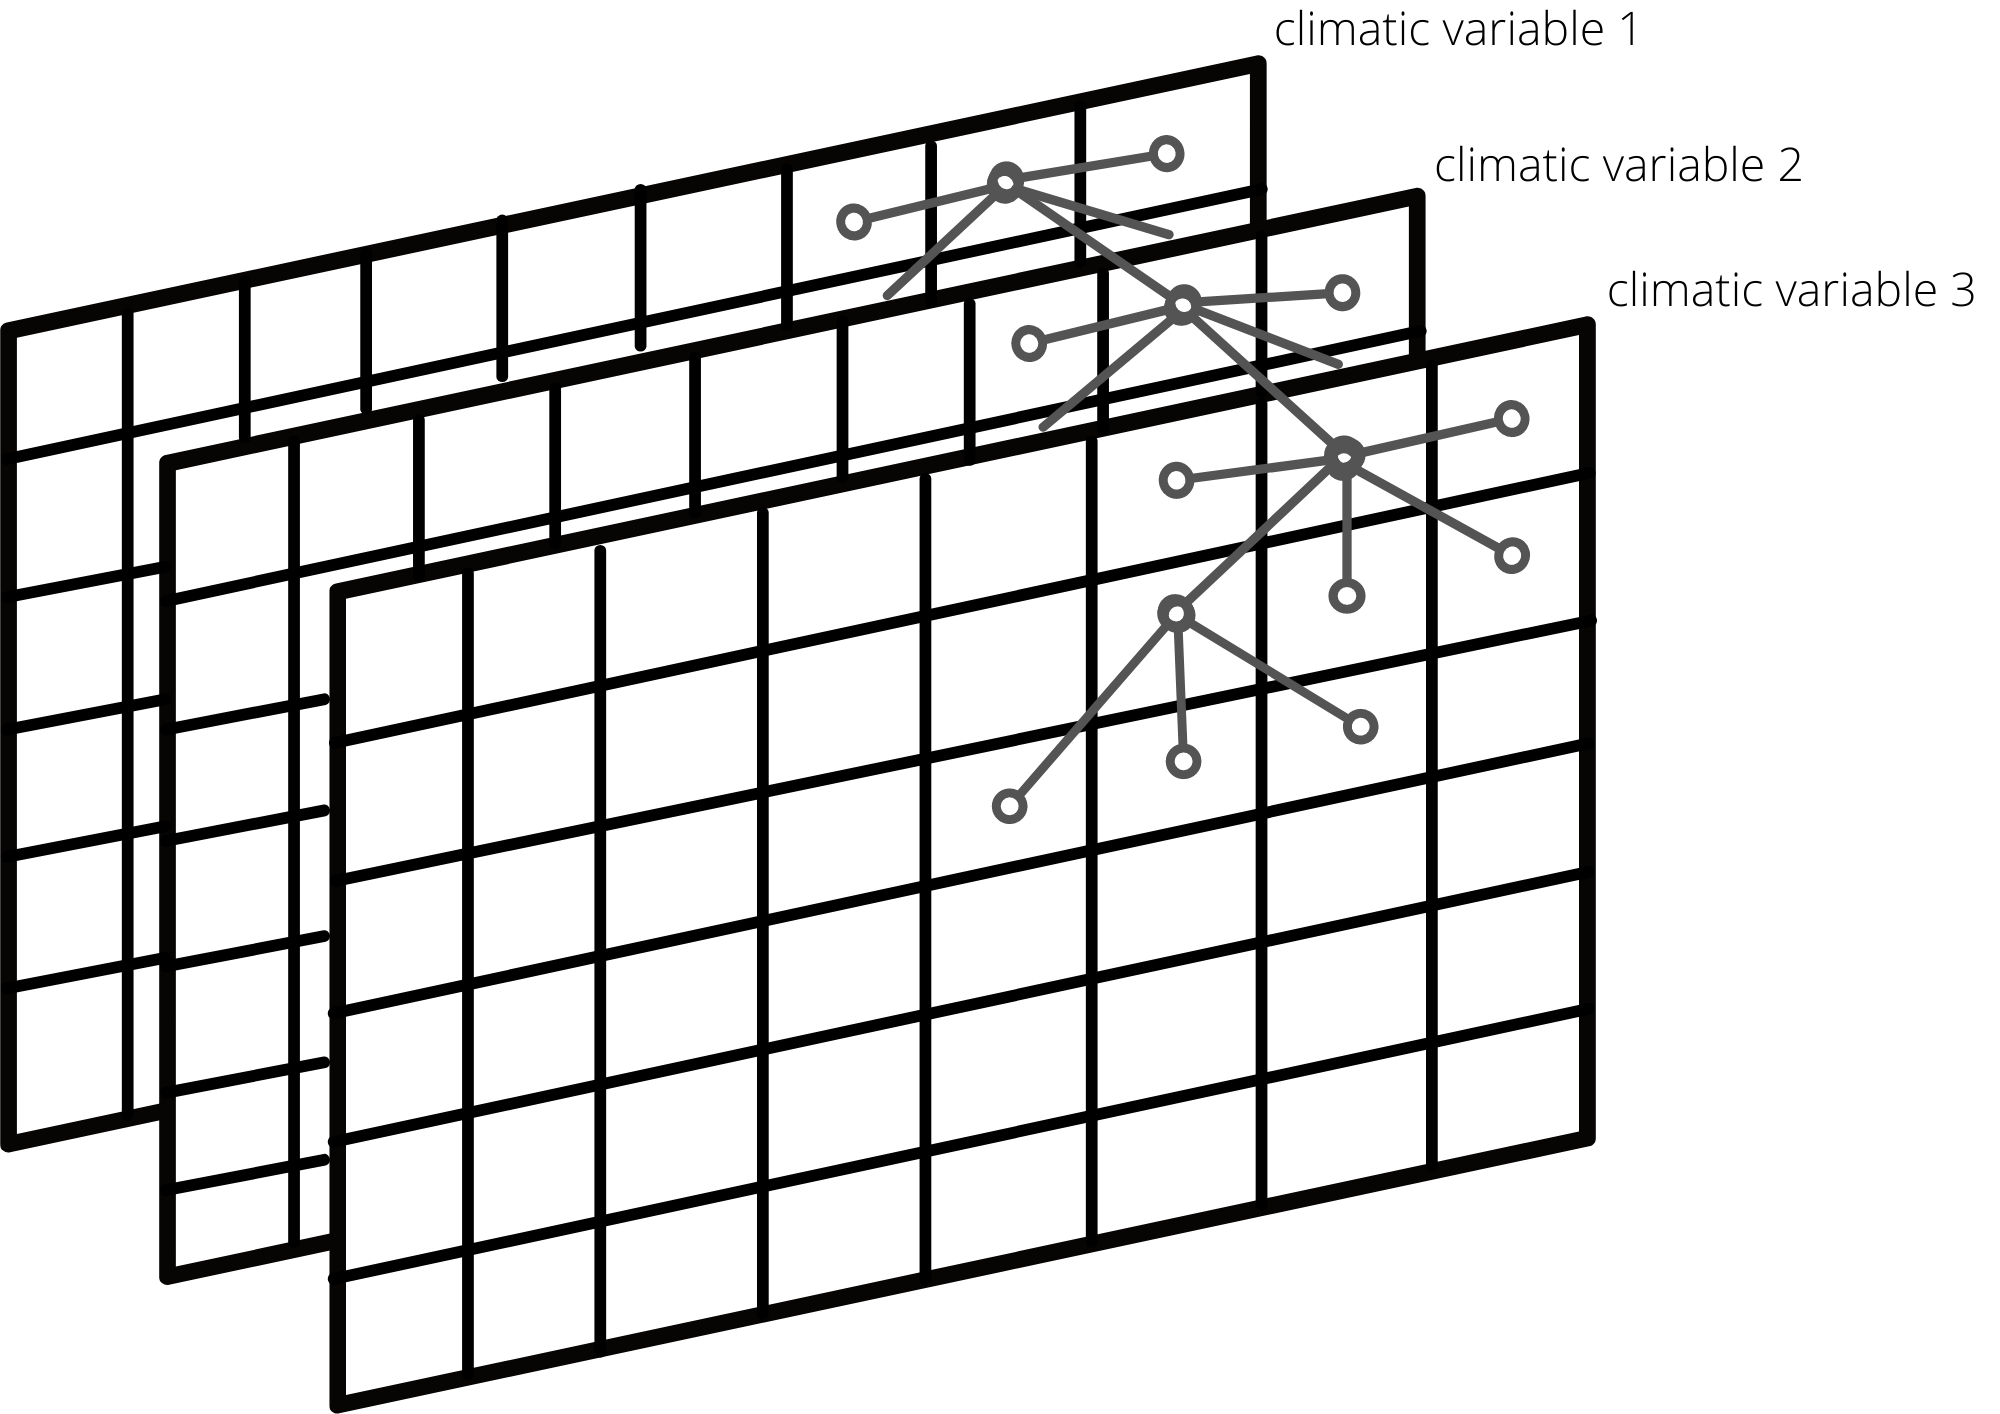
\includegraphics[scale=0.17]{figures/climate variable 1 (1).png} \\ Graph attention principle}
\end{minipage}
\hfill
\begin{minipage}[h]{0.49\linewidth}
\center{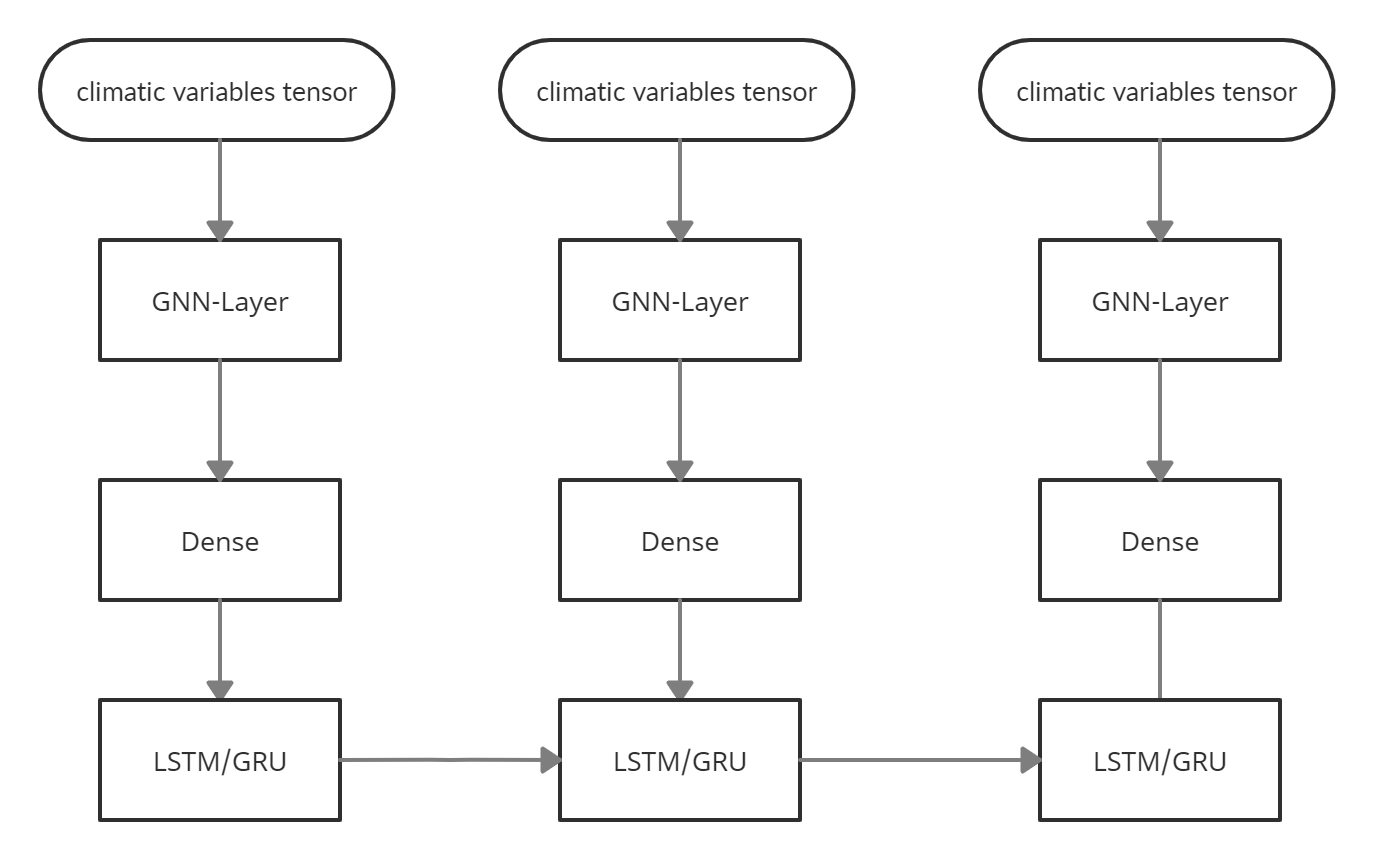
\includegraphics[scale=0.13]{figures/HailNet architecture (1).png} \\ Resulting architecture}
\end{minipage}
\end{figure}

Necessary hails conditions are combination of different climatic variables.
\end{frame}
%----------------------------------------------------------------------------------------------------------


\end{document} 